\renewcommand{\theequation}{\theenumi}
\renewcommand{\thefigure}{\theenumi}
\renewcommand{\thetable}{\theenumi}
\begin{enumerate}[label=\thesection.\arabic*.,ref=\thesection.\theenumi]
\numberwithin{equation}{enumi}
\numberwithin{figure}{enumi}
\numberwithin{table}{enumi}

\item The probability that a given positive integer lying between 1 and 100 (both inclusive) is NOT divisible by 2,3 or 5 is \dots
\\
\solution


    \begin{definition}[Characteristic Function]
    The function $\phi_X(t) = E\brak{e^{itX}}$ is called the characteristic function (cf ) of random variable $X$.
    \label{transform/1/def:characterstic_function}
   \end{definition}
   \begin{proposition}[Properties of a Characteristic function]
   All cf’s have the following properties:\\
   \begin{enumerate}
       \item $\phi_X(-t) =\overline{\phi_X(t)}$ (complex conjugate)
       \item  $\phi_{-X}(t) = \overline{\phi_X(t)}$  
   \end{enumerate}
   \label{transform/1/prop:properties_of_cf}
   \end{proposition}
   \begin{proposition}[Cf of sum of independent r.v.’s]
    If $X$ and $Y$ are independent, then
    \begin{align}
        \phi_{X+Y}(t) = \phi_X(t)\times\phi_Y(t)
    \end{align}
    \label{transform/1/prop:Sum_of_independent_cvs}
   \end{proposition}
   Let $X$ be the given random variable and let $Y$  and $-X$ have the same distribution.
   \begin{enumerate}
       \item \begin{align} [\phi_X(t)]^2 &= \phi_X(t)\times\phi_X(t) \\
                   &= \phi_{2X}(t) & & \text{(by  \ref{transform/1/prop:Sum_of_independent_cvs})}
   \end{align}
   Thus, $f(t) = [\phi(t)]^2$ is a characteristic function of random variable $2X$.
   \item \begin{align} |\phi_X(t)|^2 &= \phi_X(t)\times\overline{\phi_X(t)} \\
                   &= \phi_X(t)\times\phi_Y(t) & & \text{(by  \ref{transform/1/prop:properties_of_cf})}\\
                   &= \phi_{X+Y}(t)
   \end{align}
   Thus, $f(t)=|\phi(t)|^2$ is a characteristic function of random variable $(X+Y)$.\\
   \item \begin{align} \phi_X(-t) &= E\brak{e^{i(-t)X}} & & \text{(by  \ref{transform/1/def:characterstic_function})} \\
                   &= E\brak{e^{it(-X)}} \\
                   &= E\brak{e^{itY}}\\
                   &= \phi_Y(t)
   \end{align}
   Thus, $f(t) = \phi(-t)$ is a characteristic function of random variable $Y$.
   \item \begin{align} \phi_X(t+1) &= E\brak{e^{i(t+1)X}}  & & \text{(by  \ref{transform/1/def:characterstic_function})} \\
   &= E\brak{e^{itX}\times e^{iX}} 
   \end{align}
   Thus, $f(t) = \phi(t+1)$ is a not a characteristic function.\\
   \end{enumerate}
   Hence, correct options are 1, 2, 3.
   
%
\item P and Q are considering to apply for a job. The probability that P applies for the job is $\dfrac{1}{4}$, the probability that P applies for the job given that Q applies for the job is $\dfrac{1}{2}$, and the probability that Q applies for the job given that P applies for the job is $\dfrac{1}{3}$. Then the probability that P does not apply for the job given that Q does not apply for the job is 

\begin{enumerate}
\begin{multicols}{4}
\setlength\itemsep{2em}

\item $
\dfrac{4}{5}
$

\item $
\dfrac{5}{6}
$

\item $
\dfrac{7}{8}
$

\item $
\dfrac{11}{12}
$

\end{multicols}
\end{enumerate}
\solution
\begin{definition}
    (Convergence in distribution)\\
    A sequence of random variables $Y$, $Y_1$, $Y_2 \ldots$   converges in distribution to a random variable $Y$, if
    \begin{align}
        \lim_{n \to \infty}F_{X_{n}} (a) = F_{X} (a)  \text{  }\forall a \in \mathbb{R}.
    \end{align}
\end{definition}
\begin{definition} \label{conv/2/def2}
    (Convergence in probability)\\
    A sequence of random variables $Y$, $Y_1$, $Y_2 \ldots$ is said to converge in probability to $Y$, if
    \begin{align}
        \lim_{n \to \infty}\pr{\abs{Y_n - Y} > \epsilon} = 0  \text{  }\forall \epsilon > 0.
    \end{align}
\end{definition}
\begin{lemma}\label{conv/2/lma1}
    If
    \begin{math}
    {Y_n} \to Y \text{ in probability, }{Y_n} \to Y \text{ in distribution.}
    \end{math}
\end{lemma}
\begin{lemma}\label{conv/2/lma3}
    (Strong Law of Large Numbers)\\ 
Let $X_1$, $X_2$, \ldots $X_n$ be i.i.d. random variables with expected value $E(X_i)=\mu < \infty$, then,
\begin{align}
%    \lim_{n \to \infty}\pr{\left|\dfrac{1}{n}\sum_{i=1}^n X_i - \mu \right|\geq \epsilon}=0
X_i \xrightarrow[]{p}\mu
\end{align}
Or, 
\begin{align}
    \dfrac{1}{n}\sum_{i=1}^n X_i \xrightarrow[]{p} \mu
\end{align}
%
\end{lemma}
\begin{lemma} \label{conv/2/lmaconda}
    If $X_i$ is a sequence of i.i.d. random variables, with
    \begin{align}
        \label{conv/2/maincondA}
        F_{X_i}(x)=F_X(x),
    \end{align}
    then,
    \begin{align}
        F_{X_i^2}(x)=F_{X^2}(x)
    \end{align}
    $\forall x \in \mathbb{R}$, where $F_{X}(x)$ is the c.d.f. of $X_i$.
\end{lemma}
\begin{proof}
% ${X_i}$ is a sequence of i.i.d. random variables, which means it satisfies the following condition.
% \begin{align}
%         F_{X_1}(x)=F_{X_2}(x)&=\ldots=F_{X_n}(x)=F_X(x) 
% \end{align}
% where $F_X(x)$ is the c.d.f. of $X_i$.
% Let $Y_i=X_i^2$. For $y \geq 0$,
\begin{align}
    F_{{X_i}^2}(y) &=\pr{X_i^2 \leq y}
%     &=\pr{Y_i \leq y}\\
%     \implies F_{Y_i}(y)
% \end{align}
% \begin{align}
    \\
    \implies F_{Y_i}(y)&=\pr{-\sqrt{y} \leq X_i \leq \sqrt{y}}\label{conv/2/eqref}\\
%     \implies F_{Y_i}(y)&=\pr{X_i \leq \sqrt{y}}-\pr{X_i \leq -\sqrt{y}}
% \end{align}
% \begin{align}
\implies   F_{{X_i}^2}(y)&=F_{X_i}(\sqrt{y})-F_{X_i}(-\sqrt{y})
\\
&= F_{X}(\sqrt{y})-F_{X}(-\sqrt{y}) 
\\
&= F_{{X}^2}(y)
\end{align}
Using \eqref{conv/2/maincondA},
% \begin{align} 
%     F_{Y_i}(y)&=F_X(\sqrt{y})-F_X(-\sqrt{y})\label{conv/2/eqY}
% \end{align}
% From \eqref{conv/2/eqY},
% \begin{align} 
%     F_{Y_1}(y)=F_{Y_2}(y)=\ldots=F_{Y_n}(y)=F_Y(y)\label{conv/2/condnA}
% \end{align}
% where $F_Y(y)$ is the c.d.f. of $Y_i=X_i^2$.
\end{proof}
\begin{corollary} \label{conv/2/xi2lma}
    If $X_i$ are i.i.d, $X_i^2$ are i.i.d.
    % \begin{align}
    %     F_{X_1,\ldots X_n}(x_1\ldots x_n)&=F_X(x_1)F_X(x_2)\ldots F_X(x_n)\label{conv/2/maincondnB}
    % \end{align} 
    % where $F_{X}(x)$ is the c.d.f. of $X_i$, then for $Y_i = X_i^2$
    % \begin{align}
    % F_{Y_1,Y_2,\dots,Y_n}&(y_1,y_2,\dots,y_n)=F_Y(y_1)F_Y(y_1)\dots F_Y(y_n)
    % \end{align}
%    where $F_Y(y)$ is the c.d.f. of 
\end{corollary}
\begin{proof}
Let $Y_i = X_i^2$.
%Now, for $y_i\geq0$, consider
\begin{multline}
    F_{Y_1,Y_2,\ldots,Y_n}(y_1,y_2,\ldots,y_n)
\\=\pr{Y_1 \leq y_1,Y_2 \leq y_2,\ldots,Y_n \leq y_n}
     \\=\pr{X_1^2 \leq y_1,X_2^2 \leq y_2,\ldots,X_n^2 \leq y_n}
    %\\=\pr{-\sqrt{y_1} \leq X_1 \leq \sqrt{y_1},\ldots,-\sqrt{y_n} \leq X_n \leq \sqrt{y_n}}
    \\ = \prod_{i=1}^{n}\sbrak{\pr{-\sqrt{y_i} \leq X_i \leq \sqrt{y_i}}}
    \\= \prod_{i=1}^{n}F_Y(y_i) 
 \end{multline}
$\implies X_i^2$ are i.i.d.
% So,
% \begin{align} \label{conv/2/condnB}
%     F_{Y_1,Y_2,\dots,Y_n}&(y_1,y_2,\dots,y_n)\nonumber \\
%     &=F_Y(y_1)F_Y(y_1)\dots F_Y(y_n)
% \end{align}
\end{proof}
% \begin{lemma} 
% If ${X_i}$ is a sequence of i.i.d. random variables, it follows that $X_i^2$ is also a sequence of i.i.d. random variables.
% \end{lemma}
% \begin{proof}
%     From Lemma \ref{conv/2/lmaconda} and Lemma \ref{conv/2/lmacondb}, $X_i^2$ is also a sequence of i.i.d. random variables.
% \end{proof}
\begin{lemma} \label{conv/2/varsum}
    If $X_1, X_2, \ldots X_n$ are independent random variables,
    \begin{align}
        \var{\sum_{i=1}^n X_i} = \sum_{i=1}^{n}\var{X_i}
    \end{align}
\end{lemma}
\begin{lemma}\label{conv/2/lma4}
    (Chebyshev's Inequality)\\
Let the random variable $X$ have a finite mean $\mu$ and a finite variance $\sigma^2$. For every $\epsilon>0$, 
\begin{align}
    \pr{\abs{X - \mu} \geq \epsilon} \leq \frac{\sigma^2}{\epsilon^2}
\end{align}
\end{lemma}
\begin{lemma}\label{conv/2/lma2}
    (Central Limit Theorem)
Let $X_1$, $X_2$, \ldots $X_n$ be i.i.d. random variables with expected value $E(X_i)=\mu < \infty$  and $0 < V(X_i)=\sigma^2 < \infty$. Then the random variable 
\begin{align}
    Z_n 
%    = \frac{\bar{x} - \mu}{\frac{\sigma}{\sqrt{n}}} 
    = \frac{\sum_{i=1}^n X_i - n\mu}{\sqrt{n}\sigma}
    \xrightarrow[]{d} \gauss{0}{1}
\end{align}
% converges in distribution to the standard normal random variable as n goes to infinity, that is
% \begin{align}
%     \lim_{n \to \infty}\pr{Z_n \leq a} = \Phi(a)   \text{        }\forall a \in \mathbb{R}.
% \end{align}
% where $\Phi(a)$ is the standard normal CDF.
\end{lemma}
\begin{enumerate}
\item 
From Lemma \ref{conv/2/xi2lma}, \{$X_i^2$\} is a sequence of i.i.d. random variables.  Hence, 
%Now, we know,
\begin{align}
    E(X_i^2)=\var{X_i}+\sbrak{\mean{X_i}}^2 = 1
\end{align}
% Putting given values, we get,
% \begin{align} 
%     E(X_i^2)&=1 \label{conv/2/muval}
% \end{align}
From Lemma \ref{conv/2/lma3},  
\begin{align} \label{conv/2/opt4}
   \dfrac{1}{n}\sum_{i=1}^n X_i^2 \xrightarrow[]{p} 1 \ne 0 
\end{align}
Therefore, option 1 is incorrect.
\item 
\begin{lemma} \label{conv/2/result2}
    Let    
    \begin{align}
        Y_n=\dfrac{1}{n^{3/4}}\sum_{i=1}^n X_i,
    \end{align}
    where $X_i$ are i.i.d.  with 
    \begin{align}
        \mean{X_i} = 0, \var{X_i} = 1
            \end{align}
        Then 
        \begin{align}
            \mean{Y_n} = 0,  \var{Y_n} = \dfrac{1}{n^{1/2}} 
                \end{align}
            
\end{lemma}

\begin{proof}
\begin{align}
    \mean{Y_n} &= \dfrac{1}{n^{3/4}}\mean{\brak{\sum_{i=1}^n X_i}} = 0
\end{align}
Since $E(X_i) = 0$. Also, from Lemma \ref{conv/2/varsum},
\begin{align}
    \var{Y_n} &= \dfrac{1}{n^{3/2}} \brak{\sum_{i=1}^n\mean{ X_i}}
    \\
    &= \dfrac{1}{n^{3/2}} \times n = \dfrac{1}{n^{1/2}}
\end{align}
  $\because \var{X_i}=1$. 
\end{proof}
Now, from Lemma \ref{conv/2/lma4} and Lemma \ref{conv/2/result2}
\begin{align}
    \lim_{n \to \infty}\pr{|Y_n-0|\geq \epsilon} &\leq \lim_{n \to \infty }\dfrac{1}{n^{1/2}\epsilon^2}\\
    &= 0
%    \implies &\lim_{n \to \infty}\pr{\left | \dfrac{1}{n^{3/4}}\sum_{i=1}^n X_i - 0 \right|\geq \epsilon}=0
\end{align}
From Definition \ref{conv/2/def2},
\begin{align}
    \dfrac{1}{n^{3/4}}\sum_{i=1}^n X_i \xrightarrow[]{p} 0
\end{align}
Thus, option 2 is correct.
\item Substituting $\mu=0$ and $\sigma=1$, in  Lemma \ref{conv/2/lma2},
\begin{align}
    Z_n &= \dfrac{1}{n^{1/2}} \sum_{i=1}^n X_i  \xrightarrow[]{d} \gauss{0}{1} \ne 0
\end{align}
% From Lemma \ref{conv/2/lma2} 
% \begin{align}
%     \dfrac{1}{n^{1/2}} \sum_{i=1}^n X_i \to  N(0,1)
% \end{align}
% whereas the option states that
% \begin{align}
%  \dfrac{1}{n^{1/2}} \sum_{i=1}^n X_i \to 0
% \end{align} 
% from Lemma \ref{conv/2/lma1}.
Therefore, option 3 is incorrect.
\item From \eqref{conv/2/opt4}, option 4 is correct.
\end{enumerate}
Therefore, options 2 and 4 are correct.
%
%
\item Out of 6 unbiased coins, 5 are tossed independently and they all result in heads. If the 6th coin is now independently tossed, the probability of getting head is:
\begin{enumerate}[label=(\alph*)]
\item 1
\item 0
\item $\frac{1}{2}$
\item $\frac{1}{6}$
\end{enumerate}
%
\solution
Define a random variable $X=\{0,1\}$ denoting the outcome of the toss of 6th coin with $X=0$ and $X=1$ representing tails and head respectively.Therefore,
\begin{align}
\pr{X=0} + \pr{X=1} &= 1\\
\pr{X=1} &= \frac{1}{2}
 \end{align}
 
Hence the correct answer is option $(\mathrm{c})$.

\item Two students are solving the same problem independently,if the probability of first one solves the problem is $\frac{3}{5}$ and the probability that the second one solves the problem is $\frac{4}{5}$ ,what is the probability that atleast one of them solves the problem?
\begin{enumerate}

\item $ \frac{17}{25}$\\
\item $\frac{19}{25}$\\
\item $ \frac{21}{25}$\\
\item $\frac{23}{25}$

\end{enumerate}
%
\solution
\input{solutions/2018/june/18.tex}
%
\item Three types of components are used in electrical circuits 1, 2, 3 as shown below in the figure
\begin{figure}[h]
    \centering
    \includegraphics[width=\columnwidth]{solutions/2016/june/118/Figures/circuits.png}
    \caption{Figure}
    \label{fig:fig_label}
\end{figure}
%
\solution
For $q_1$, the truth table
\begin{table}[h]
    \centering
    \begin{tabular}{|c|c|c|c|}
    \hline
         $A$ & $B$ & $C$ & $(AB) + C$ \\
         \hline
         1 &1  & 0 &1\\\hline
         1&1&1&1\\\hline
         0&1&1&1\\\hline
         0&0&1&1\\\hline
         1&0&1&1\\
    \hline
    \end{tabular}
    \caption{Circuit 1 working}
    \label{june2016-118:tab:my_label}
\end{table}
Multiplying and adding probability for each case of $q_1$ gives us the value of $q_1$ as
\begin{align}
    q_1 = p^3-2p^2+1
\end{align}
For $q_2$, the truth table
\begin{table}[h]
    \centering
    \begin{tabular}{|c|c|c|c|}
    \hline
         $A$ & $B$ & $C$ & $(A+B)C$ \\
         \hline
         1&1&1&1\\ \hline
         1&0&1&1\\\hline
         0&1&1&1\\
    \hline
    \end{tabular}
    \caption{Circuit 2 working}
    \label{june2016-118:tab:table2}
\end{table}
Multiplying and adding probability for each case of $q_2$ gives us the value of $q_2$ as
\begin{align}
    q_2 = p^3-p^2-p+1
\end{align}
For $q_3$, the truth table
\begin{table}[h]
    \centering
    \begin{tabular}{|c|c|c|c|}
    \hline
         $A$ & $B$ & $C$ & $A + B + C$ \\
         \hline
         1&0&0&1\\\hline
         0&1&0&1\\\hline
         0&0&1&1\\\hline
         1&1&0&1\\\hline
         1&0&1&1\\\hline
         0&1&1&1\\\hline
         1&1&1&1\\
    \hline
    \end{tabular}
    \caption{Circuit 3 working}
    \label{june2016-118:tab:table3}
\end{table}
Multiplying and adding probability for each case of $q_3$ gives us the value of $q_3$ as
\begin{align}
    q_3 = 1-p^3
\end{align}
%%
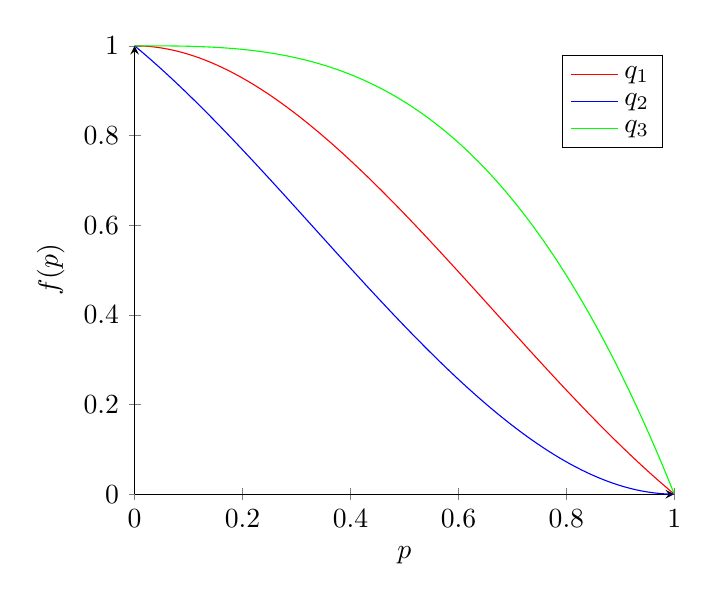
\begin{tikzpicture}
\begin{axis}[
    axis lines = left,
    xlabel = $p$,
    ylabel = {$f(p)$},
]
\addplot [
    domain=0:1, 
    samples=100, 
    color=red,
]
{x^3-2*x^2+1};
\addlegendentry{$q_1$}
\addplot [
    domain=0:1, 
    samples=100, 
    color=blue,
    ]
    {x^3-x^2-x+1};
\addlegendentry{$q_2$}
\addplot [
    domain=0:1, 
    samples=100, 
    color=green,
]
{1-x^3};
\addlegendentry{$q_3$}
\end{axis}
\end{tikzpicture}
\begin{align}
    \therefore q_3>q_1>q_2
\end{align}
Hence \textbf{Option 1} is correct
\end{enumerate}